\chapter{Big Table}
\label{bigTable}

\section{Einführung}
Täglich kommen mehrere Petabytes an Daten von über 60 Google Anwendungen zusammen. Dafür verantwortlich sind mehr als 1000 Computer die untereinander vernetzt sind. Um diese Daten verwalten zu können wurde Bigtable ins Leben gerufen. Das Ziel der Datenbank war es in vielen Bereichen angewendet werden zu können. Dazu sollte es skalierbar sein sowie eine hohe Performance und Verfügbarkeit besitzen.


\section{Datenmodell}
Bigtable ist eine verteilte, persistente multidimensionale sortierte Map. Diese Map ist indexiert über eine row key, column key und einem timestamp. Jeder Wert in dieser Map ist ein Array mit Bytes. Das folgende Datenmodell soll eine Speicherung von Webseiten veranschaulichen.

\begin{figure}[!htpb]
	\centering
	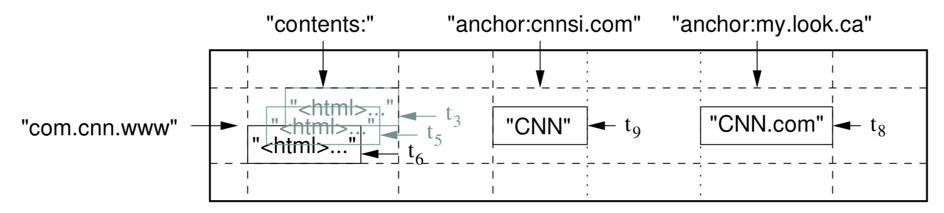
\includegraphics[]{pics/bigtable_schema.png}
	\figuresource{https://static.googleusercontent.com/media/research.google.com/de//archive/bigtable-osdi06.pdf}
	\caption {Tabellen Beispiel}	
\end{figure}

Das Datenmodell besteht aus zwei Familien dem Inhalt und den Ankerpunkten. Die erste Familie beinhaltet den Inhalt der Webseite, mit drei unterschiedlichen Zeitstempeln (t3, t5, t6). Drei unterschiedliche Zeitstempel bedeutet, dass die Website www.cnn.com in drei unterschiedlichen Versionen abgespeichert wurde. Die Anker Familie beinhaltet jeweils nur eine Version. Den Anker mit \glqq CNN.com \grqq mit dem Zeitstempel t8 und dem Anker \glqq CNN \grqq mit dem Zeitstempel t9. 
 
\paragraph{Rows}
Bigtable speichert Daten in lexikograhischer Reihenfolge und sortiert diese nach Zeilen. Eine row range beinhaltet alle gleichnamigen URL’s, so dass alle mit der gleichen Domain zusammen abgespeichert werden. Das vereinfacht die Analyse und das Hosting der gleichnamigen Domains und macht dies zudem effizienter.

\paragraph{Column families}
Verschiedene column keys werden in eine gemeinsame Gruppe gespeichert. Das nennt man column families. Alle Daten, welche in der gleichen Gruppe gespeichert werden sind vom gleichen Typ. Bevor Daten in einer Gruppe gespeichert werden können, muss diese column family als erstes erstellt werden.

\paragraph{Timestamp}
Jede Zelle in Bigtable kann mehrere Versionen der gleichen Daten beinhalten. Dieser Versionen werden indexiert durch den Zeitstempel (timestamp). Der Zeitstempel ist bis auf die Micro Sekunde genau. Durch die \glqq two per-column-family \grqq kann der Benutzer festlegen, wie viele Versionen der gleichen Daten gespeichert werden sollen. Alle weiteren Versionen werden automatisch gelöscht.

\paragraph{API}
Die API von Bigtable ermöglicht das erstellen und löschen von Tabellen und Spaltennamen, sowie das ändern von Tabellen, Cluster und Metadaten einer Spaltenfamilie. Das folgende Codebeispiel wurde in C++ geschrieben und verändert den Inhalt der Tabelle Webtable. 

\begin{figure}[!htpb]
	\centering
	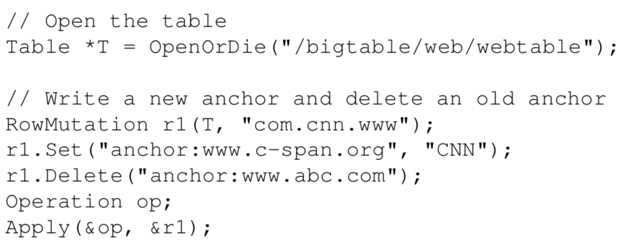
\includegraphics[]{pics/bigtable_api.png}
	\figuresource{https://static.googleusercontent.com/media/research.google.com/de//archive/bigtable-osdi06.pdf}
	\caption {Zugriffs Beispiel mit der BigTable API}
\end{figure}

Der Code verändert die Spalte \glqq com.cnn.www \grqq und fügt einen neuen Anker hinzu. Im nächsten Schritt wird ein vorhandener Anker \glqq anchor:www.abc.com \grqq gelöscht und festgeschrieben.


\paragraph{Building Blocks}
Bigtable ist auf mehreren anderen Teilen der Google-Infrastruktur aufgebaut. Zum Beispiel benutzt Bigtable das verteilte Google File System (GFS). Welches für die Speicherung von Logs und Daten verantwortlich ist. Ein Bigtable Cluster operiert typischerweise auf einem verteilten Pool von Computern. Auf diesem Pool laufen eine breite Sparte von verschiedenen Anwendungen. Bigtable basiert auf einem Cluster Management System für Zeit-Planung-Jobs, Ressourcenmanagements auf geteilten Computern, agieren mit Computerfehlern und dem Anzeigen des Computer Status. Das SSTable Format stellt eine persistente, geordnete unveränderliche Abbildung von Schlüsseln zu Werten zur Verfügung, wobei sowohl Schlüssel als auch Werte willkürliche Bytefolgen sind. Operationen werden bereitgestellt, um den Wert zu suchen, der einem bestimmten Schlüssel zugeordnet ist.

\paragraph{Implementation}
Bigtable besteht aus drei Haupt Komponenten, einer Bibliothek, einem Master Server und vielen weiteren tablet servern. Die Bibliothek ist in jeden Client verlinkt, somit kann der Client auf alle Funktionen zugreifen. Der Master Server wird zufällig ausgewählt. Dieser teilt den tablet servern die tablets zu. Außerdem ist  er für die Verteilung der Lasten  und  für die garbage collection zuständig. Sobald eine Tabelle zu groß wird, wird diese von einem tablet server gesplittet. So wird sichergestellt, dass eine Tabelle nie größer als 100-200 MB ist.

\paragraph{Tablet location}
Um Daten zu speichern, verwendet Google bei Bigtable eine \glqq three-level hirarchy \grqq. Das erste Level ist eine Datei, welches auch das Chubby file genannt wird, dort wird der Speicherort des root tablets hinterlegt. Das root tablet beinhaltet alle Speicherorte aller tablets in einer METADATA Tabelle. Das spezielle an dieser Tabelle ist, dass egal wie groß sie wird, diese niemals geteilt wird. Somit wird sichergestellt, dass die \glqq three-level hirarchy \grqq eingehalten wird. Die METADATA Tabellen speichern die Orte aller anderen tablets in einer Tabelle ab.

\paragraph{Tablet Zuweisung}
Jedes tablet ist zu einem Zeitpunkt immer nur einem tablet server zugeordnet. Der Master server verfolgt die lebenden tablet server und die aktuell zugeordneten tablets zu den tablet servern inklusive aller unzugeordneten tablet servern.
Beim Start einer Bigtable führt der Master Server folgende Schritte aus:

\begin{enumerate}
	\item Wählt einen einzigartigen Master Lock in Chubby
	\item Scannt die Server Verzeichnisse um die lebenden tablet server zu finden
	\item Kommuniziert mit den vorhandenen tablet server um bereits zugeordnete tablets zu identifizieren
	\item Master scannt METADATA Tabelle um die vorhandene Zugehörigkeiten zu lernen
\end{enumerate}

\paragraph{Tablet serving}
Ein persistenter Zustand eines tablets wird in GFS gespeichert. Alle Updates werden auf \glqq well-formed \grqq geprüft und anschließend in einem commit-log gespeichert. Die neusten Updates werden in eine memtable gespeichert, ältere updates werden in die SSTable geschrieben. Wenn Daten aus dem tablet server abgefragt werden muss ein merge zwischen den neuen Daten in der memtable sowie den älteren Daten in der SSTable erstellt werden.

\paragraph{Compaction}
Je mehr Daten gespeichert werden, umso größer wird die memtable. Damit diese tabelle nicht zu groß wird, gibt es ein \glqq minor compaction \grqq. Diese Funktion friert eine memtable ein sobald diese eine bestimmte Größe erreicht hat und erstellt eine neue memtable. Die gefrorene memtable wird zu einer SSTable konvertiert. Je mehr Daten gespeichert werden, desto unordentlicher wird die Ansammlung von SSTable. Um die SSTable zu sortieren wird periodisch ein \glqq merging compaction \grqq ausgeführt. Dies strukturiert die SSTable neu und es werden Ressourcen, durch die Löschung von Daten, freigegeben. Außerdem werden gelöschte Daten endgültig gelöscht, das ist wichtig für Services, welche sensible Daten beinhalten.

\section{Refinments}
Um die hohe Performance, Verfügbarkeit und Zuverlässigkeit beizubehalten, werden einige Verbesserungen (refinments) benötigt.

\paragraph{Lokale Gruppen}
Gruppierung erspart Zugriffszeit. Zum Beispiel bei dem Datenmodell Webseite. Die \glqq page metadate \grqq und \glqq content \grqq der Webseite werden in einer anderen Gruppe gespeichert. So muss eine Anwendung, welche nur die Metadaten möchte, nicht durch den kompletten Inhalte einer Seite iterieren.
Zudem gibt es Tuningparameter, welche bestimmten ob Daten in den Arbeitsspeicher geladen werden um die Zugriffszeit zu minimieren.

\paragraph{Kompression}
Ein Benutzer kann selbst bestimmen ob eine SSTable komprimiert wird und falls ja, in welchem Ausmaß. Jeder SSTable Block kann einzeln ausgewählt werden. Für die Komprimierung kommen die  Verfahren Bentley und McLlroy’s zum Einsatz. Diese können mit 100-200Mb/s kodiert und mit 400-1000 MB/s enkodiert werden.

\paragraph{Caching für Lesezugriffe}
Für das Caching von Lesezugriffe gibt es zwei Verfahren. Der Scan Cache (high-level), speichert key-value Paare und liefert eine SSTable zurück. Das Block Cache (lower-level) Verfahren speichert SSTable Blocks, die von der GFS gelesen werden.

\paragraph{Bloom Filter}
Benutzer legt selbst fest ob ein Filter zum Einsatz kommt. Der Vorteil eines Filters liegt darin, dass wenn Daten gesucht werden, nicht jede SSTable nach den bestimmten Daten durchsucht werden muss. Ein Bloom Filter erlaubt es, nach einer bestimmten Art von row/column-Paaren zu fragen, ob diese in einer SSTable gespeichert sind.

\paragraph{Beschleunigte tablet Wiederherstellung}
Wenn der Master ein tablet von einem Server zu einem anderen Server verschiebt, führt der Ursprungsserver erst ein \glqq minor compaction \grqq aus um die Ladezeit für den neuen tablet server zu verkürzen.

\paragraph{Unveränderlichkeit ausnutzen}
Es können nur Daten verändert, welche in der memtable stehen. Daten in der SSTable können nicht verändert werden. Das macht man sich zu nutzen indem man keine Synchronisation braucht, wenn auf die Daten zugegriffen wird. Memtable sind die einzigen Daten auf die man schreiben kann und gleichzeitig lesen. Damit es zu keinen Konflikten kommt, setzt Bigtable hier auf \glqq Copy-on-write \grqq. 

\section{Performance Auswertung}
\begin{figure}[!htpb]
	\centering
	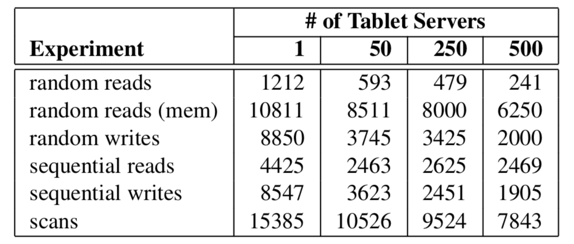
\includegraphics[]{pics/bigtable_performance.png}
	\figuresource{https://static.googleusercontent.com/media/research.google.com/de//archive/bigtable-osdi06.pdf}
	\caption {Percormance Übersicht}	
\end{figure}
Die Performance wird hauptsächlich durch die verwendete CPU (2ghz) begrenzt. Zudem kann man erkennen, dass bei einem tablet server der Durchsatz bei ca. 75MB/s liegt (1000 bytes * 64 KB Block size = 75 MB/s). Damit der Durchsatz bei einem Single tablet server erhöht wird, wird die die SSTable größe in der regel von 64KB auf 8kb gesenkt. 
Zudem wird erkannt, dass der Durchsatz nicht linear ansteigt. Bei einer Erhöhung der tablet server von eins auf 500 liegt die Erhöhung des Durchsatzes bei gerade mal dem 300 fachen (10811 / (500 * 6250) = 350). Diese Begrenzung liegt wie bei einem tablet server an der CPU der tablet servern.
